\chapter{Mechanics} % (fold)
\label{chap:mechanics}
	When the ball is dropped it has to be caught in the first bounce. 
	For this, a mechanical structure holds an actuator that moves an arm which catches the ball as instructed by the FPGA.

	\section{Design} % (fold)
	\label{sec:mechanics_design}
		The physical implementation of the project is divided in three parts.

		First, the platform where the sensors are located. 
		The physical platform area will be a flat area of approximately $40\times40\,\si{\centi\meter}$.
		The dimensions were chosen like this due to this size was found appropriately for the projects goals according to the ball's size and the actuator's size and characteristics.
		This platform is decided to be an aluminum sheet due to two reasons: 
		\begin{itemize}
			\item Metal sheets usually have homogeneous mechanical properties and this especially important for this project because the same propagation waves speed is searched.
			\item Inside the metals, aluminum was chosen for stock reasons and easy manufacturing. 
		\end{itemize}
		This platform is separated from the down surface with plastics legs in the corners that let the waves, first reach the sensors and then dissipate through them.

		Second the structure is able to hold the motor and the arm. This design enables the user to change the height of the actuator in order to test the machine in different conditions. 
		%This capability will be used to measure the reaction speed of the project. 
		The structure has to be strong and rigid enough so that it does not deform more than an specified precision.

		Third, the actuator enables movement of an arm that will catch the ball when required. 
		This actuator needs to be precise enough to satisfy the precision criteria of the project, in this case, less than the ping pong ball diameter. 
			
		Having this requirements in mind, the arm was decided to have only one servo motor for simplicity reasons and as a prove of concept. 
		The inverse kinematics was really easy to calculate and much simpler in the assembly and maintenance.
	% section design (end)
	
	\section{Manufacturing} % (fold)
	\label{sec:mechanics_manufacturing}
		As explained before an aluminum sheet was used for the platform for its homogeneous properties and availability. 
		In the platform two deflections are found: the one due to the gravity and the one due to the hit of the ball. 
		The sheet finally was 3\si{mm} thick because of the availability and due to, for a square of 400\si{mm} side, the finite element method (FEM) studies showed that the deformation produced by its own weight is in another order of magnitude, so this deflection does not affect to the real measurement. 
		In the figure \ref{fig:FEM} a hit of 1\si{N} force is shown and it shows approximately $5.1e-02\si{mm}$ of deformation in the direction of the hit.
		\begin{figure}[htb]
			\begin{center}
				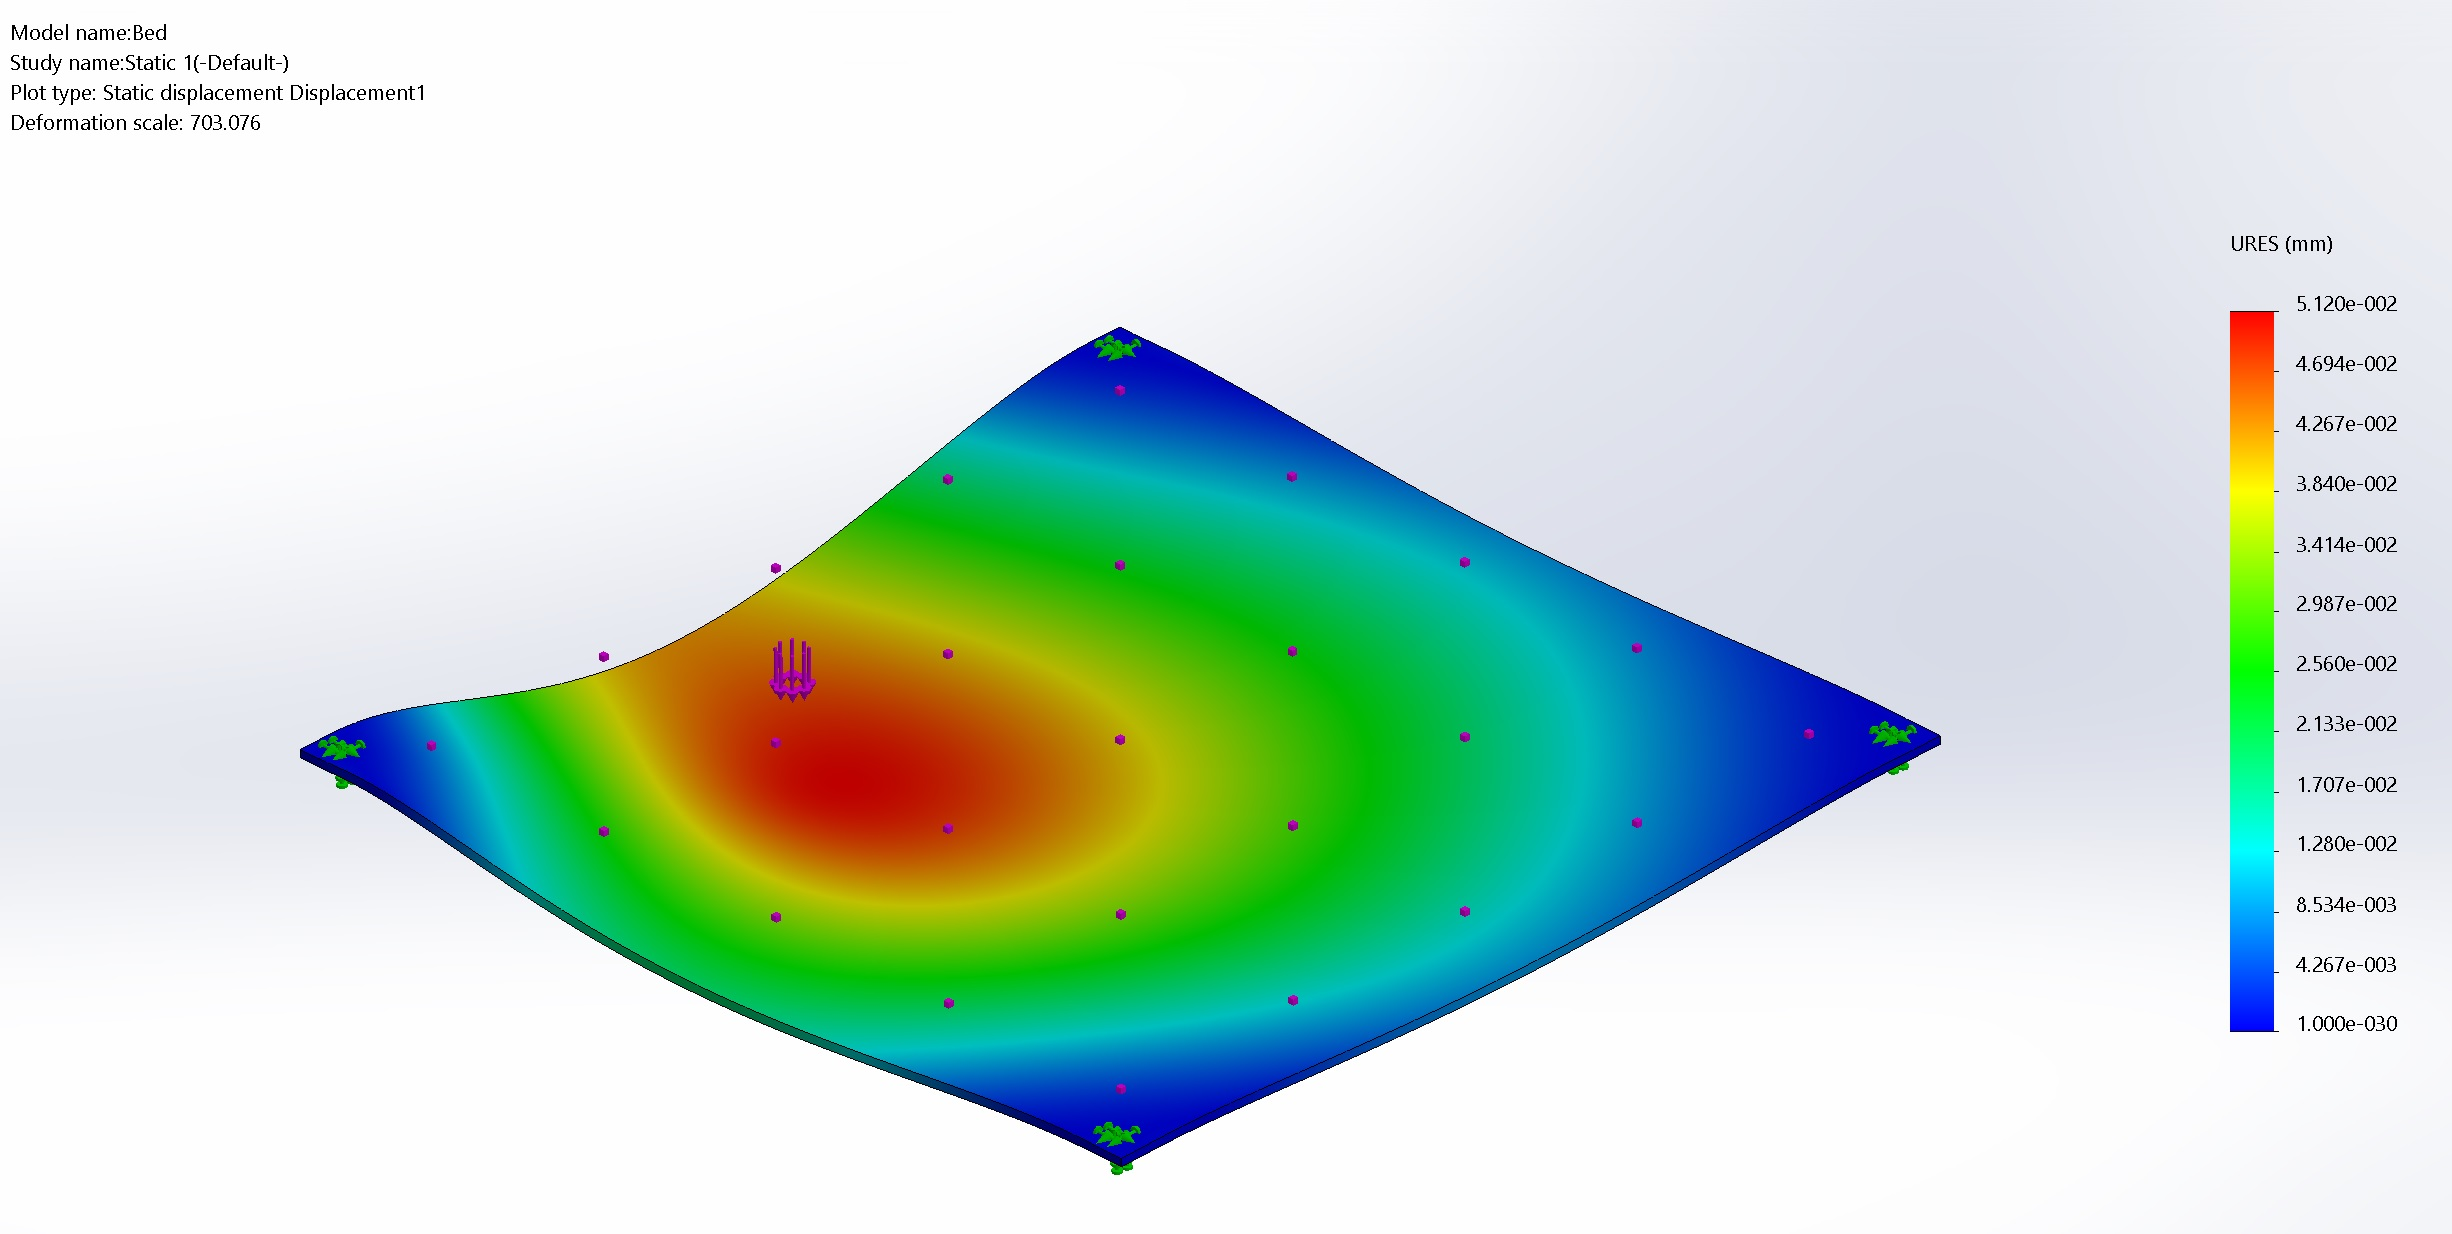
\includegraphics[width=.8\textwidth]{figures/FEM}
			\end{center}
			\caption{FEM static analysis for a hit of 1\si{N} in the platform.}
			\label{fig:FEM}
		\end{figure}
		Due to the requirement to make the structure with different positions for the motor a tower like structure with holes is made. The size of it demands for manufacture with the laser cutting technology. 
		The available laser cutter enables to make parts up to 800\si{mm} so the total structure's height was chosen to be 400\si{mm}, the same as the side of the platform. 
		Based on this size, an $L$-structure was designed to be strong in the X an Y stresses while, to absorbs the torque, two squads were put in the bottom and the top.
		Also four legs are assembled in the structure to give more stability. They are the same part has one of the squads so not other parts are designed assuring easy for big lots.
		
		The arm is designed to reduce as much as possible the deformation during the movement and when the ball is caught. For manufacture the arm along with the squads. A Fused Deposition Modeling (FDM) 3D printer was used due to the possibilities of the shape it lets and also because of the availability. Finally, the screws and nuts were chosen based on what was in stock at the time. In the figure \ref{fig:render2} a render of the final design is shown.

		\begin{figure}[htb]
			\begin{center}
				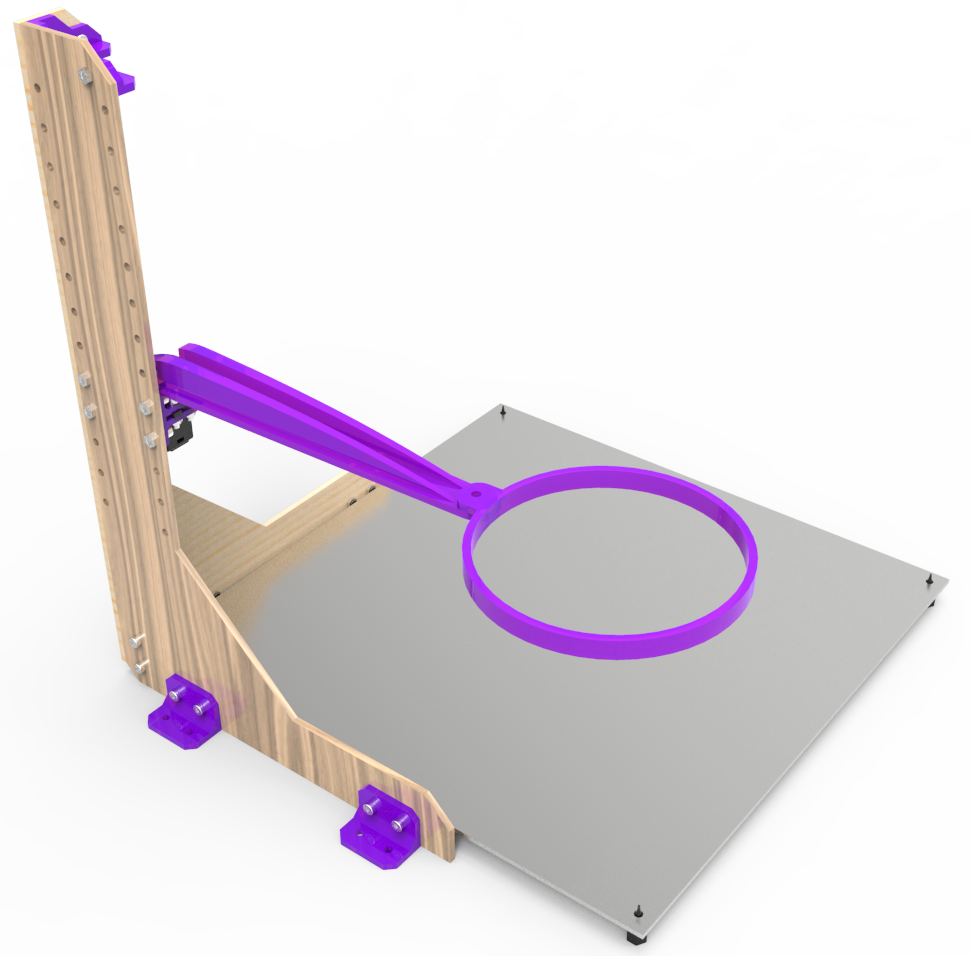
\includegraphics[width=.8\textwidth]{figures/render2}
			\end{center}
			\caption{Render of the final design.}
			\label{fig:render2}
		\end{figure}
	% section manufacturing (end)

	\section{Conclusions} % (fold)
	\label{sec:mechanics_conclusions}
		The assembly of the whole project was as expected and no modifications were required. Some troubles were found while mounting the servo because it was difficult to assembly it, but not impossible. That is a point to be improved.

		On the other hand, the structure responded as expected and it enables preforming all the test necessaries. In the figure \ref{fig:photo1} the final assemble prototype is shown.

		\begin{figure}[htb]
			\begin{center}
				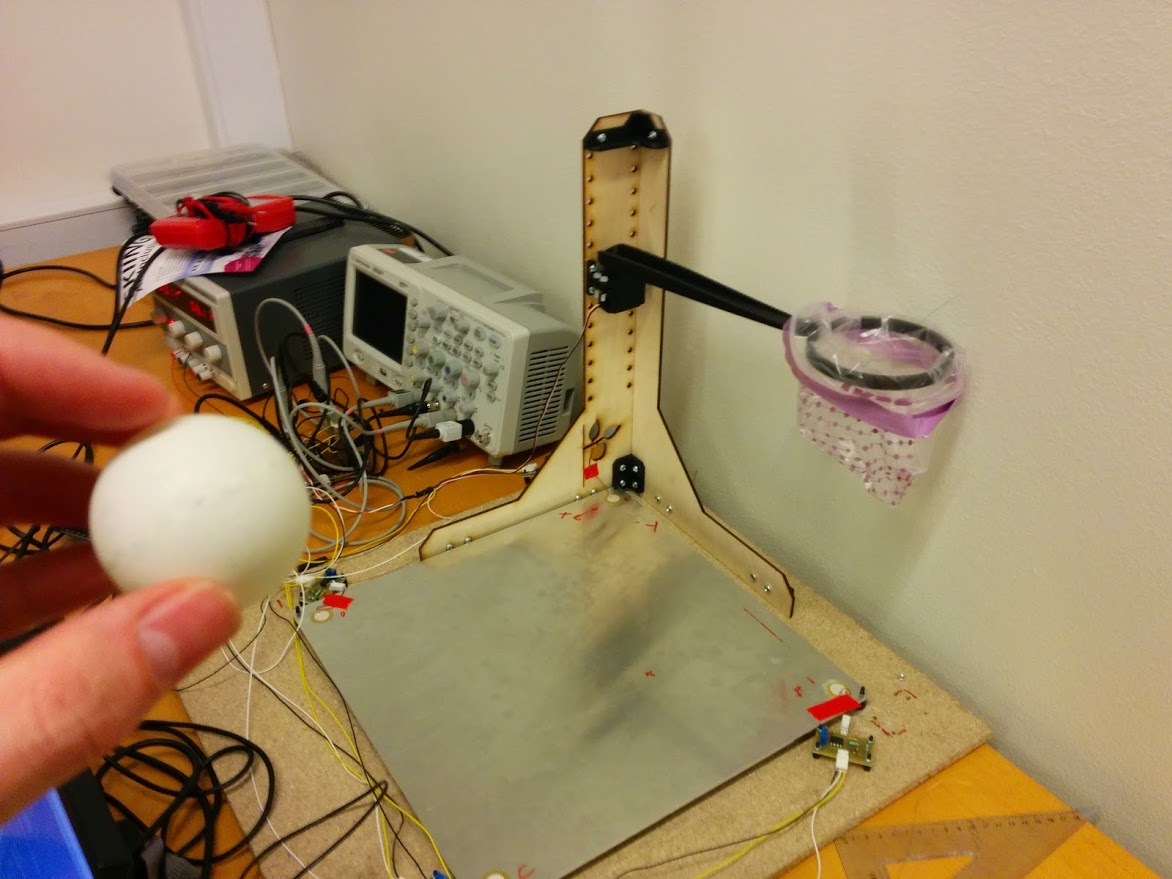
\includegraphics[width=.8\textwidth]{figures/photo1}
			\end{center}
			\caption{Photo of the final assembled prototype.}
			\label{fig:photo1}
		\end{figure}
	% section conclusions (end)
% chapter chapter_name (end)